\chapter{ER random graphs}

\resp{Vicentini Gioele}

\section{Introduction to the ER study}
The aim here is to replicate the results obtained via simulations of the graphs in figure 3 of the original paper. The study is of both the diameter of an ER network for different wiring probabilities $p$ and the size of its LCC. Finally, we find the size of the LCC for different values of the percolation probability $p_{ext}$ by obtaining the relative optimal value of the probability $p_{op}$ that a link has enough entangled pairs to perform a functional connection. This pairs of values $(p_{ext}, p_{op})$ are the ones satisfying the condition $l(p_{op}) = D(p_{op}p_{ext})$ and were obtained from the simulation results.

\section{Hysteresis in the first order phase transition}
The first step is to obtain the minimum value of $p_{op}$ for a given value of $p_{ext}$. In the paper an exponential distribution of qbit pairs is assumed, $g(n) = \exp\left( -n \right)$ such that the functional dependence of $l_{op}$ on $p_{op}$ is:
\begin{align}
    l_{op} &= n_{op}^{1/\alpha} \\
    p_{op} &= \int_{n_{op}}^{+\infty} dn A\exp\left(-n/\langle n\rangle\right)dn  \\
    &= -A\langle n \rangle \left[0 - \exp\left(-n_{op}/\langle n\rangle\right)\right] \\
    l_{op}&= \left[-\langle n\rangle\log\left(\frac{p_{op}}{A\langle n \rangle}\right)\right]^{1/\alpha}  \\
    A:\quad & \int_{0}^{+\infty} dn A\exp\left(-n/\langle n\rangle\right)dn = 1 \\
    A &= \frac{1}{\langle n \rangle}
\end{align}
Since the condition is $l_{op}(p_{op}) = D(p_{op}p_{ext})$, for a given value of $p_{ext}$ we can find $p_{op}$.

So the idea is:
\begin{itemize}
    \item Find the average diameter of the ER graphs of some finite ensemble for varying $p$
    \item Get the corresponding critical value for $p_{op}$ (more than one for the hysteresis region)
    \item Calculate the average backbone for all pairs $(p_{ext}, p_{op})$
\end{itemize}
But we encounter right away the first problem: the histeresis region appears only with really high numbers of nodes $N \sim 10^5$, which is far too much for my laptop since a fundamental part of the analysis consists in calculating over and over the diameter of a huge network (and multiple times). I wasn't able to replicate the results in time and it seems that the transition to the coexistance of phases is quite sharp, since even at $5\cdot 10^4$ nodes it wasn't showing up.
In order to widen the coexistance region, the following results were calculated for $\alpha=2$.

The results are in graphs \autoref{fig:ER_Robustness}.
\begin{figure}
    \centering
    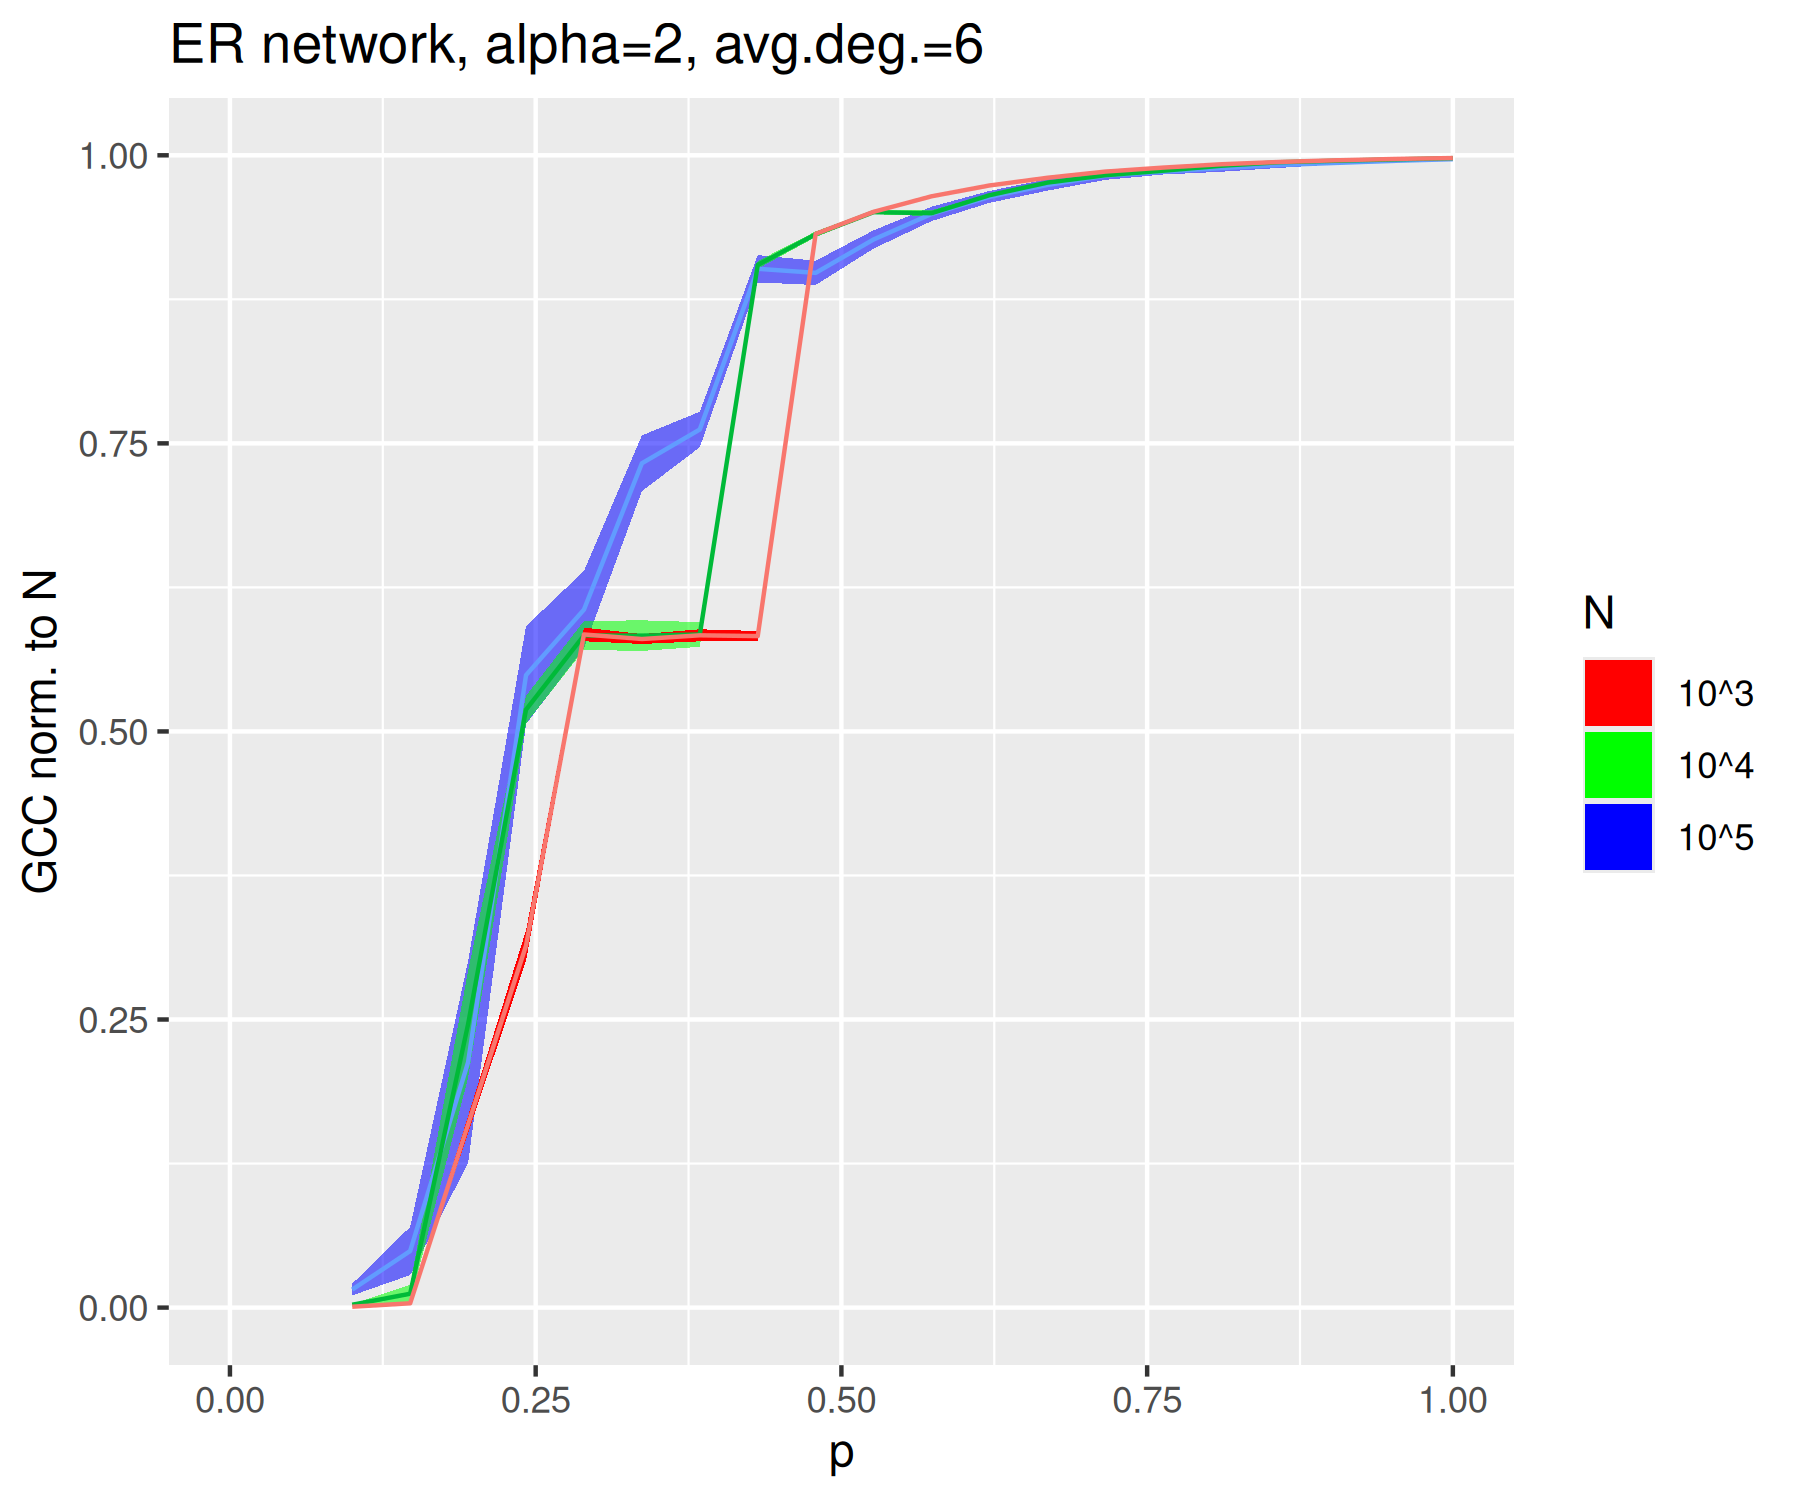
\includegraphics[width=0.7\linewidth]{images/ER_GCC.png}
    \includegraphics[width=0.7\linewidth]{images/ER_Rob.png}
    \caption{Results on ER networks: average diameter under percolation and $l_{op}$, size of the GCC. No hysteresis can be seen as the critical condition $l_{op}(p_{op})=D(p)$ is hardly ever met if $N<10^5$.}
    \label{fig:ER_Robustness}
\end{figure}
\newpage